\documentclass[12pt]{article}
\usepackage[utf8]{inputenc}
\usepackage[automark]{scrlayer-scrpage}
\usepackage[T1]{fontenc}
\usepackage[pdftex]{graphicx,color}
\usepackage{subcaption}
\usepackage{url}
\usepackage[pdftex,pdfpagelabels]{hyperref}
\usepackage[section,boxed]{algorithm}
\usepackage{algpseudocode}
\usepackage{amsmath}
\usepackage{amssymb}
\usepackage{amsthm}
\usepackage{lmodern}
\pagestyle{scrheadings}
\ofoot{}\cfoot{}\ifoot{}
\lehead{\pagemark}
\rehead{\slshape\leftmark}
\lohead{\slshape\leftmark}
\rohead{\pagemark}
\newtheorem{definition}{Definition}
\newtheorem{theorem}{Theorem}
\usepackage{blindtext}
\usepackage[margin=1in]{geometry}
\usepackage{amsmath,amsthm,amssymb}
\usepackage{graphicx}
\newcommand{\N}{\mathbb{N}}
\newcommand{\Z}{\mathbb{Z}}
\newcommand{\R}{\mathbb{R}}
\newcommand{\C}{\mathbb{C}}

\begin{document}
% --------------------------------------------------------------
%                         Title Page
% --------------------------------------------------------------
\title{Solutions for Sheet 1}
\author{Raphael Wude, Martin Brückmann, Claude Jordan, Daniel Degenstein\\ \\
\textsc{Pattern Matching and Machine Learning} \\
\textsc{for Audio Signal Processing}}
\maketitle

% --------------------------------------------------------------
%                         Task 1.1
% --------------------------------------------------------------
\section*{Task 1.1}
\begin{itemize}
    \item[(a)]
    $z = (\frac{\sqrt{2}}{2}+i\frac{\sqrt{2}}{2})^{3} = (\frac{\sqrt{2}}{2})^{3} + 3(\frac{\sqrt{2}}{2})^{2}(i\frac{\sqrt{2}}{2}) + 3(\frac{\sqrt{2}}{2})(i\frac{\sqrt{2}}{2})^{2} + (i\frac{\sqrt{2}}{2})^{3} = \frac{1}{2}(-1+i)\sqrt{2}=\frac{1}{\sqrt{2}}(-1+i)=-\frac{1}{\sqrt{2}}+\frac{1}{\sqrt{2}}i$\\\\
    $|z|=\sqrt{(-\frac{1}{\sqrt{2}})^{2}+(\frac{1}{\sqrt{2}})^{2}}=1$\\\\
    $cos\varphi=\frac{Re[z]}{|z|}=\frac{-\frac{1}{\sqrt{2}}}{1}=-\frac{1}{\sqrt{2}}$\\\\
    $\varphi=cos^{-1}(-\frac{1}{\sqrt{2}})=\frac{3\pi}{4}$\\\\
    $\Rightarrow z=|z|\cdot e^{i\varphi}=e^{\frac{3\pi i}{4}}$

    \item[(b)]
    Write down the following complex number in Cartesian coordinates:
   $$z = \frac{e^{\frac{5\pi}{3}i}}{e^{\frac{4}{3}\pi i} \cdot 2 e^{\frac{11}{6}\pi i}}.$$
\begin{align*}
   z &= \frac{e^{\frac{5\pi}{3}i}}{e^{\frac{4}{3}\pi i} \cdot 2 e^{\frac{11}{6}\pi i}} = \frac{1}{2} e^{\left(\frac{5}{3} - \frac{4}{3} - \frac{11}{6}\right)\pi i} \\
   &= \frac{1}{2} e^{\frac{3}{2}\pi i}
\end{align*}
With Euler's Formula $e^{iz} = cos(z) + i \cdot sin(z)$ and $cos\left(\frac{3 \pi}{2}\right) = 0$ and $sin\left(\frac{3 \pi}{2}\right) = -1$:
\begin{align*}
   z &= \frac{1}{2} e^{\frac{3}{2}\pi i} = \frac{1}{2} \cdot (-i) = 0 - \frac{1}{2} i
\end{align*}
So the complex number in Cartesian coordinates is: $z =0 - \frac{1}{2} i$
\newpage
    \item[(c)]
    Calculate explicitly:
    $Re[5e^{\frac{\pi}{4}i}+\sqrt{2}e^{\pi i}]$.
    \begin{align*}
        Re\left[5e^{\frac{\pi}{4}i}+\sqrt{2}e^{\pi i}\right] &= Re\left[5\left(\frac{\sqrt{2}}{2} + i \cdot \frac{\sqrt{2}}{2} \right)+\sqrt{2}\cdot (-1)\right] \\
        &= Re \left[5 \cdot \frac{\sqrt{2}}{2} - \sqrt{2} + 5 \cdot \frac{\sqrt{2}}{2}i \right] = Re \left[\frac{3}{2} \sqrt{2} + \frac{5 \sqrt{2}}{2} i \right] \\
        &= \frac{3}{2} \sqrt{2}
    \end{align*}
    The real part of the complex number $5e^{\frac{\pi}{4}i}+\sqrt{2}e^{\pi i}$ is $\frac{3}{2} \sqrt{2}$.
    \item[(d)]
    Using Euler's Formula, prove the following statement:

$sin(z)^2 + cos(z)^2 = 1, z \in \mathbb{C}$\\
Proof:\\
Euler's formula is as follows: $e^{iz} = cos(z) + i \cdot sin(z), z \in \mathbb{C}$\\
For the opposite angle $-z$, we have $e^{-iz} = cos(z) - i \cdot sin(z)$\\
With these two, we can derive the following for $i \cdot sin(z), cos(z)$:\\
$i \cdot sin(z) = e^{iz} - cos(z) = cos(z) - e^{-iz}$\\
$cos(z) = e^{iz} - i \cdot sin(z) = e^{-iz} + i \cdot sin(z)$\\
And by plugging in, we can write $sin(z), cos(z)$ only in terms of $e^{iz}, e^{-iz}$:\\
$cos(z) = e^{iz} - i \cdot sin(z) = e^{iz} - cos(z) + e^{-iz} = \frac{e^{iz} + e^{-iz}}{2}$\\
$sin(z) = \frac{e^{iz} - cos(z)}{i} = \frac{e^{iz} - e^{-iz} - i \cdot sin(z)}{i} =\frac{e^{iz} - e^{-iz}}{2i}$\\
All that's left is to square and plug in once more:\\
$sin(z)^2 = \frac{1}{-4}((e^{iz})^{2} - 2e^{iz}e^{-iz} + (e^{-iz})^2)$\\
$cos(z)^2 = \frac{1}{4}((e^{iz})^{2} + 2e^{iz}e^{-iz} + (e^{-iz})^{2})$\\
$sin(z)^{2} + cos(z)^{2} = \frac{1}{4}4e^{iz}e^{-iz} = 1$\\

\end{itemize}
% --------------------------------------------------------------
%                         Task 1.2
% --------------------------------------------------------------
\section*{Task 1.2}
\begin{figure}[H]
    \centering
    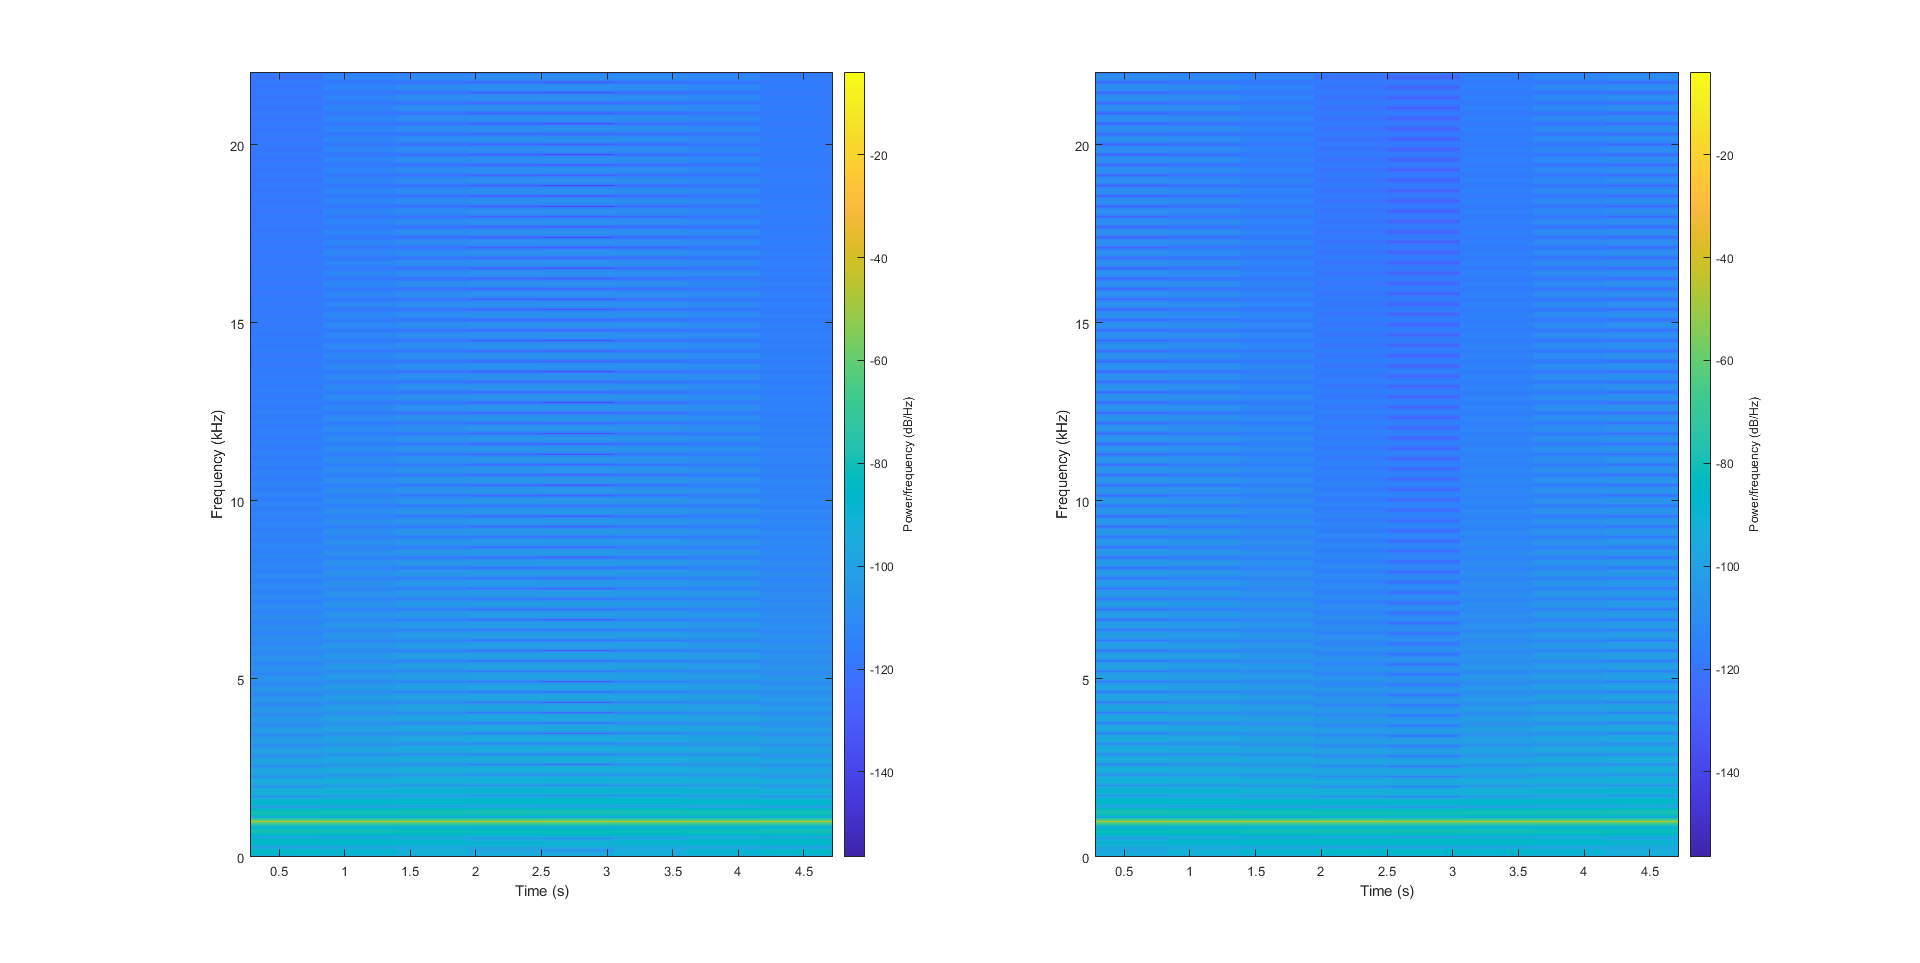
\includegraphics[width=1.1\textwidth]{Spectrograms.png}
    \caption{time-frequency representations for the sine wave (left) and cosine wave (right)}
    \label{abb}
\end{figure}
If we look at both spectrograms in Figure \ref{abb}, we see that there are no differences between the two waves. This is due to the fact that a cosine wave is only a phase-shifted sine wave. Therefore, both time-frequency representations are the same.

\end{document}
